% PREAMBLE
\documentclass[a4paper, 12pt, titlepage, openany]{book}
\usepackage[top=1in,right=2.5cm,left=2.5cm,bottom=1in]{geometry}
\usepackage{mathptm}
\usepackage{hyperref}
\usepackage{epsfig} 
\usepackage{tipa}
\usepackage{subfigure}
\usepackage{footnote}
\usepackage[gnu]{newtitle} 
\usepackage{fancyheadings} 
\usepackage[numbers,square]{natbib}
\pagestyle{empty}
\usepackage[grey,times]{honoursThesis}
\usepackage{listings}

% TITLE PAGE
\title{Anonymous Go-Kart: Specification Report}
\date{\today}

\author{
  {Henry Jenkins, Wim Looman, Simon Richards, Zachary Taylor}\vspace{0.1cm}\\
    Department of Computer and Electrical Engineering\vspace{0.1cm}\\
    University of Canterbury, Christchurch, New Zealand}

\begin{document}
\maketitle
% I removed the next line to remove blank page after title page - Henry
\pagenumbering{roman}
\frontmatter
\thispagestyle{empty}
\begin{center}\section*{Abstract}\end{center}
\thispagestyle{empty}

This project looks at transforming a provided electrically powered go-kart into an autonomous vehicle capable of driving and navigation without human assistance. We have three main goals for this project. The first is to integrate a drive by wire system into the go-kart, so that it can be easily controlled by a laptop. The second is to develop a code that makes use of on-board sensors and the drive by wire system to execute a simple autonomous algorithm. This algorithm will follow a marker allowing the kart to automatically follow a person or vehicle. Finally while we wish to progress further and develop a program that will allow the kart to detect obstacles and navigate between GPS points we believe that we will not have sufficient time to make any significant progress towards this final goal. To date we have developed schematics and detailed plans for the drive by wire system. We have begun order parts and will begin putting together the systems in the next few weeks.

\vfill
  \begin{figure}[h]
    \centering
    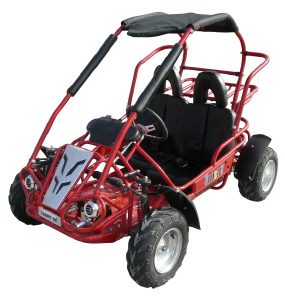
\includegraphics{../../Images/hh80h.jpg}
    \label{gokart}
  \end{figure}

% The abstract should be written assuming no other part of the report is read. A
% short statement about what your project is, what its goals are, progress made
% to date, and outlook for completing major project tasks is really what we’re
% looking for.



\pagestyle{fancy}

\renewcommand{\chaptermark}[1]
{\markboth{\uppercase{\thechapter.\ #1}}{}}
%\renewcommand{\sectionmark}[1]
%{\markboth{\uppercase{\thesection.\ #1}}{}} % Changed so the section is on both. - Wim
\setlength{\headrulewidth}{0.5pt} \setlength{\footrulewidth}{0pt}

\newcommand{\helv}{\fontfamily{pag}\fontseries{b}\fontsize{9}{11}\selectfont}

% Changed these so page numbers are always on the right and the headers are
% always on the left. - Wim
\lhead[\helv \leftmark]{\helv \leftmark}
\rhead[\helv \thepage]{\helv \thepage}
\cfoot[]{}

\newpage
\tableofcontents
\newpage

\mainmatter
    \chapter{Project Overview}

    \chapter{Project Overview}

    \chapter{Approach and Preliminary Design}

\section{Approach}
Soon after receiving this project it was decided that we would break the project up into a series of smaller projects that we would complete in series. This decision was made after we realised that the transformation of the provided go-kart to a fully working autonomous vehicle was a goal that we would likely be unable to achieve in the time allotted

The idea behind the separation into several smaller projects is that if we tried to do everything at once we would not finish the project and what we would have done would be useless to future groups. This is because most sections of the system would not be operating correctly and those that were would be interfacing with unfinished systems on a low level making them difficult to use. By dividing the project into a series of modules with each one being completed and communicating with the next via a simple well documented interface we ensured that we would have developed a strong base which future teams could easily interface with and build upon with minimal repeating of work. The sub-projects we have divided this project into are outlined below
\begin{description}
\item[Drive by wire] This is the conversion of the go-kart from a largely mechanical system to something that can be controlled by a laptop. 
Sensor interfacing- In this module the sensors the system will use to perceive the karts state and the world around it are chosen. After selection they are attached to the kart and interfaced with the control system. 

\item[High level control of systems] The drive by wire module will provide functions that directly relate to the karts systems such as the angle of the steering wheel, braking force and accelerator position. This module would seek to write functions that can be used to move away from having to deal with these low level operations. An example of this would be a function that would use the brake, accelerator and a Hall Effect sensor to allow the user to simply give the speed they wished the kart to travel at.  

\item[Simple autonomous behaviour] this would be the development of a straight forward and quick to implement program for autonomous control of the kart. A sensor on the front of the kart would detect a marker and move to be within a set distance of it. In this way the go-kart could autonomously follow a person or another vehicle

\item[Complex autonomous behaviour] this module would see the integration of path finding into the autonomous go-karts system enabling it to operate as a fully-fledged autonomous vehicle able to operate without any form of human interaction or control. When completed it would allow the go-kart to autonomously find its way to a GPS location avoiding obstacles along the way.
\end{description}

\section{Brake}

The go-kart's brakes will be controlled via a linear actuator. This will be
connected by removing the brake pedal and connecting the actuator directly to
the input of the hydraulic brake systems. It was decided to use the existing
hydraulic system rather than attach a controlled actuator directly to the brake
disk. This was done as it allowed the system to be attached and operated with
minimal modifications to the existing kart. Another reason this decision was
made is that actuators with relatively low force and large travel were much more
readily available and cheaper then those with small movement and high force and
the existing hydraulic system already converted this large movement into the
high force required resulting in a cheaper system. Through rough testing it was
determined that a human could apply approximately 300 N to the brake pedal. The
leverage in the brake pedal was estimated at be roughly a 2 to 1 system. This
meant the ideal actuator had to provide 600 N of force to operate the brakes. To
go from full off to fully on the actuator required 30 mm of travel.

The actuator selected to power the brake was a 24V Warner linear m-track1. Its
specifications deviated from our requirements slightly. The actuator had 100mm
of travel more then three times the required making it longer then necessary.
However space was not an issue so this was not seen as a problem. The actuator
could only produce 450 N of force, it has yet to be seen how fast a deceleration
this will allow however as 600N is the maximum a human could reasonably apply we
are confident 450N will be sufficient. In the unlikely event this force proves
too small in testing the large travel of the actuator means it can instead be
mounted to the brake pedal using the leverage to give the required force. The
actuator moves at 15mm per second under load. This means that from off to full
lock takes 2 seconds. This speed is a lot slower then desired however the brake
pads do not actually touch the brake during the first half of the travel. This
dead zone is there to prevent drivers accidentally applying the brakes and to
accommodate different thickness brake pads as they wear. If the servo is
recalibrated on a regular bases this dead zone can be all but removed allowing
full brake control in a second. The main driving decision in the purchase of the
actuator was price. The actuator was an end of line product that had been
heavily discounted to sell this meant that it only cost \$110 NZD including
shipping to New Zealand from America. An actuator of similar specification could
not be located for less then \$220 in the US or within New Zealand for less then
\$300.

\section{Steering}

The steering on the go-kart operates on a rack and pinion system. The steering
wheel rotates from lock to lock in 270 degrees. At rest on concrete the wheel
requires 7 Nm to turn, this value represents a worst case scenario with
significantly less force required when the kart is moving or on grass. Initially
a servo was going to be used to drive the steering wheel however servos with the
ability to produce 7Nm of continuous torque at a reasonable speed were found to
be both difficult to locate and prohibitively expensive (\$500+). Instead a
system of a DC motor, gearbox and encoder is to be used. For the motor to be
attached the steering column needs to be removed and the output of the gearbox
will drive the pinion directly with the motor bolted in the space left by the
removed column. %Not necessarily but it reads well.

The motor system selected for use in the go-kart is the IG52-04 52mm gear motor.
It comes with a 1:353 gearbox and a Hall Effect encoder attached to a second
rear output shaft on the motor. This motor produces 10 Nm of continuous torque
which will allow it to easily turn the wheel. Its gearbox output rotates at 10
RPM allowing it to travel from lock to lock in 4.5 seconds. A concern with using
this motor is that it has the ability when stalled to produce a peak torque of
up to 100 Nm. This high torque has the potential to damage the steering system
or the gearbox which is only rated for peak torques of 30 Nm. Because of this it
must be ensured that the wheel is never driven right up till the end of its
travel to prevent the motor stalling against the end and generating these
forces. The encoder must be calibrated upon each setup of the system. This is
because the encoder only outputs change in rotation and the rack may be in any
position when the system is initialised. Because of this limit switches will be
placed on small plates attached to the rack shaft to indicate when it has
reached the end of its travel. On start up the motor will locate both limit
switches to calibrate its location. These limit switches will also act as kill
switches during operation to prevent the motor reaching the end of its travel.

\section{Controlling the motor and actuator}

Both systems operate on 24V. This was done as the go-kart already had a 24V rail
for driving the main motor. Using the same voltage saves money and simplifies
the design as it precludes the need for converters that would have to be capable
of the 5A peak currents produced by the system. Both systems are controlled
through an H-Bridge interfaced with a SAM7 processor connected to a can bus.
These SAM7s take care of all the low level control required to operate the
drives allowing the main control computer to operate them at a high level with
instructions that corresponds to desired behaviour rather low level drive
operation.

The SAM7 responsible for steering will take the desired wheel angle as an input
from the can bus. It will also track the encoder's output to calculate the
turning angle. Running a PID controller between the setpoint and current value
it will send the PID loops output as a PWM signal to the H-bridge.

The design of the linear actuator is similar. The SAM7 will be passed the
current and desired speeds of the go-kart. From this and the voltage output by
the potentiometer built into the linear actuator the error in the actuator's
location will be found. Again a PID controller will drive a PWM signal to the
H-bridge controlling the actuator.

\section{High-level logic and control}

For high level control it was decided to design a system where the go-kart can
be fully controlled by a laptop using a simple USB interface.  There are a few
reasons behind this decision, the biggest one would have to be the much nicer
programming environment presented on a standard PC.  A large availability of
higher level languages and better libraries for any low level stuff that may be
required means that it will be easier to design and build the control system.

This also makes it much simpler to interface to a set of more complex sensors,
doing any sort of computer vision system on an embedded system would require a
lot more effort to design, build and test than doing the same on a standard PC.

To support this simple USB interface a modular design will be employed, a
general overview of the approach can be seen in Fig. \ref{can-design}.

\begin{figure}
  \centering
  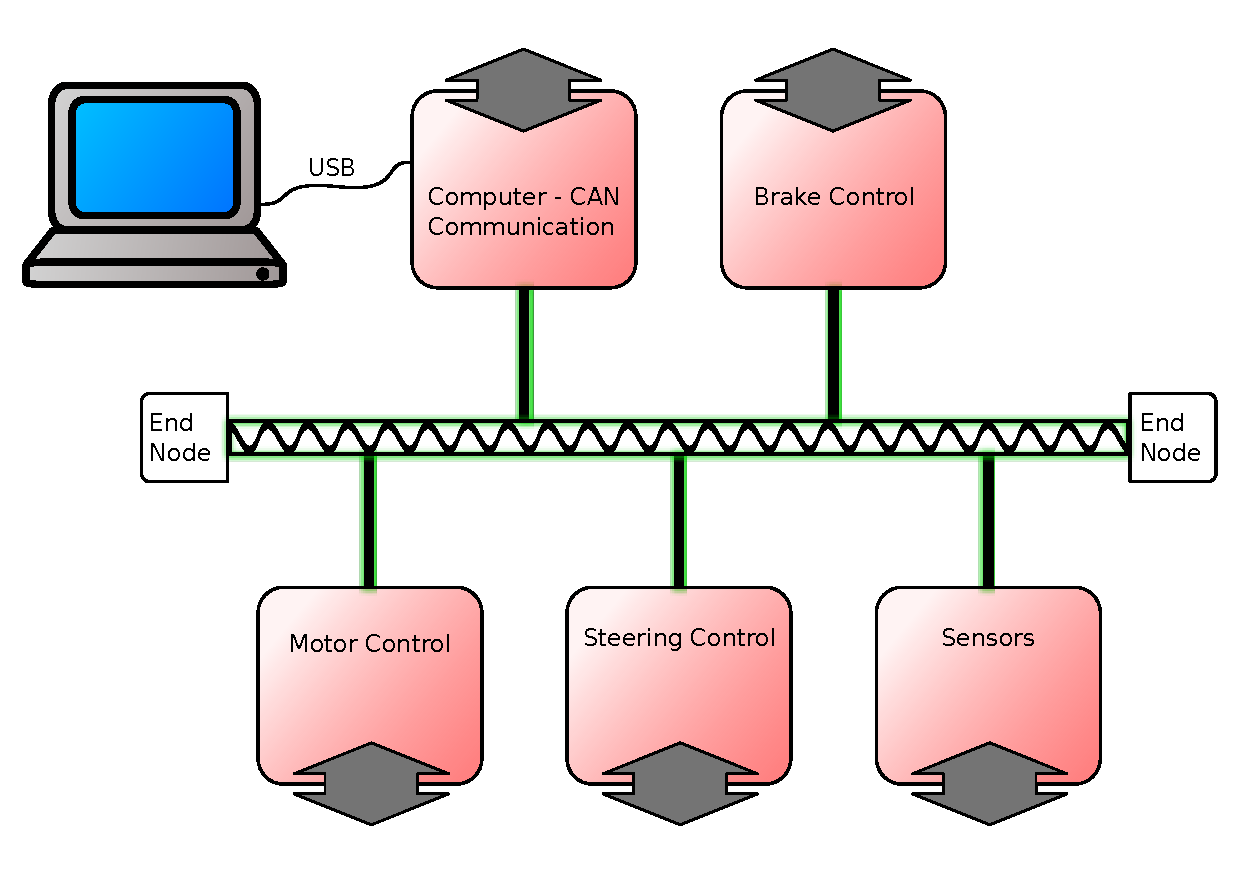
\includegraphics[width=0.8\textwidth]{../../Images/can_diagram.pdf}
  \caption{Basic go-kart control system overview.\label{can-design}}
\end{figure}

\subsection{SAM7X}

\subsection{CAN bus}


    \chapter{Budget and Timeline Summary}
% Give a summary of actual and anticipated purchases (include shipping and
% delivery). to met s and results are encouraged, regardless of success. A
% timeline summary from start of the project to completion should be included –
% a Gantt chart may be appropriate.

\section{Budget}
After building preliminary system designs, a bill of materials including parts
costs has been composed. Where possible pieces have been from either Digikey,
Element 14, Mouser or estimated if the components will come from the ECE store.

Currently both the Gear Motor with Encoder and the Linear actuator have been
ordered as they have a month lead time coming from the USA. All other components
will be ordered within the next two weeks.

{\small
\begin{tabular}{ | l | l | p{.40\textwidth} | l | l | l | l | }
\hline
 & Part Number & Description & Qty & Cost & Subtotal \\
\hline
\multirow{4}{*}{Steering} & IG52 – 04 & 24VDC 10rpm Gear Motor with Encoder & 1 & \$185.00 & \$185.00 \\
 & Shipping & Gear Motor Shipping & 1 & \$75.00 & \$75.00 \\
 &  & Motor Driver & 1 & \$0.00 & \$0.00 \\
 &  & Mounting Bracket & 1 & \$50.00 & \$50.00 \\
\hline
\multirow{4}{*}{Breaking} & 5 1752 & 4 inch stroke 100lb 24VDC Linear actuator  & 1 & \$50.00 & \$50.00 \\
 & Shipping & Linear actuator Shipping & 1 & \$50.00 & \$50.00 \\
 &  & Mounting Bracket & 1 & \$50.00 & \$50.00 \\
\hline
\multirow{3}{*}{Accelerator} & ATMEGA8L & Interface to go-kart power control & 1 & \$5.16 & \$5.16 \\
 & LM317KCS & IC VOLT REG POS ADJ & 1 & \$1.13 & \$1.13 \\
 &  & PCB & 1 & \$20.00 & \$20.00 \\
\hline
\multirow{11}{*}{CAN Bus} & PL-STP6-0 & 0.5M Cat6 STP Lead (CAN Bus) & 3 & \$4.50 & \$13.50 \\
 & PL-STP6-1 & 1.0M Cat6 STP Lead (CAN Bus) & 1 & \$5.70 & \$5.70 \\
 & SS60000-009G & RJ45 JACK (CAN Input/output) & 10 & \$4.96 & \$49.60 \\
 & Header 10X2 & Header, 10-Pin, Dual row (JTAG ) & 5 & \$1.00 & \$5.00 \\
 & fdd8445 & MOSFET 40V, 50A, 8.7mΩ & 5 & \$2.00 & \$10.00 \\
 & SW-PB & Switch (Reset) & 5 & \$3.00 & \$15.00 \\
 & AT91SAM7X & Microcontroller (CAN Controller) & 5 & \$19.37 & \$96.85 \\
 & ATA6660 & High Speed CAN Transceiver & 5 & \$2.47 & \$12.35 \\
 & AE9925-ND & USB Type B connector & 5 & \$1.52 & \$7.60 \\
 & MCP130T-300I & Microcontroller Supervisory Circuit & 5 & \$0.76 & \$3.80 \\
 &  & PCB Manufacture and shipping & 1 & \$217.00 & \$217.00 \\
\hline
\multirow{4}{*}{Other} &  & Misc Components (Diodes, Resistors, Capacitors, Wire, Headers) & 1 & \$60.00 & \$60.00 \\
 & Shipping & Shipping from Digikey and Element14 & 1 & \$30.00 & \$30.00 \\
\hline
 &  &  &  & Total & \$1,012.69 \\
\hline
\end{tabular}
}



\section{Timeline}
The Autonomous Go-Kart project has been broken down into small sections then time
allocations have been put next to each task. Where possible we have put in
dependencies between each of the tasks. However this model of only starting one
task once the previous one has been completed is not very accurate. For example
the control software has been represented as requiring the hardware to be
complete. Actually the control software will be started much before the hardware
is complete.

To make sure the project deadlines are met, milestones have been added for each
assessment or hand in item. 

%if we are on track
%Second section of Autonomous work and how it pushes past hand in


  \begin{figure}[h]
    \centering
    %\includegraphics[width=0.5\textwidth]{Images/TB9100.jpg}
    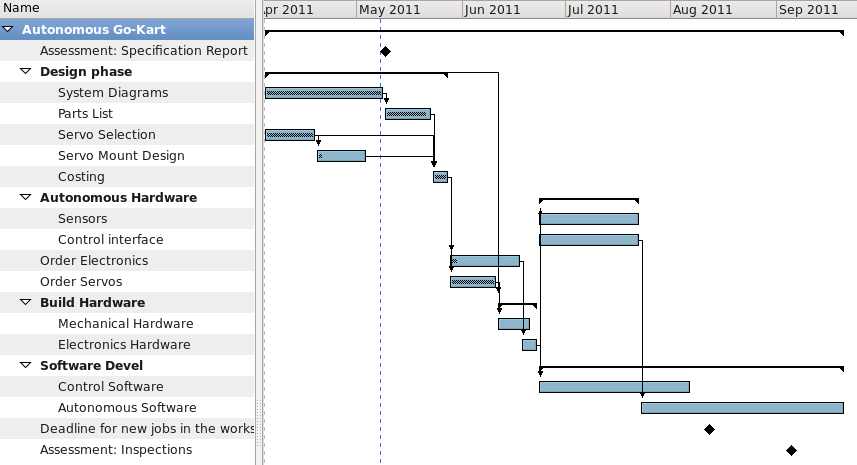
\includegraphics[width=1.0\textwidth]{Images/Gantt.png}
    \caption{Gantt chart of the Autonomous Go-Kart project}
    \label{gantt_chart}
  \end{figure}

    \chapter{Project Risks and Conclusions}

The project was divided up into several modules as was outlined in the approach and preliminary design section. The current status and our feelings on the ability to complete these modules is outlined below.

\begin{description}
\item[Drive by wire] For this system we have already completed a fairly detailed preliminary design on how the system will work and the different sections will communicate and have begun ordering the required parts. We are all fairly confident that we will have this section completed well within the allotted time for the project

\item[Sensor interfacing] While there are no concrete plans for this module as of right now the group has began to research which sensors would best suit the application and are within our budget. The group has also looked into the best way to interface them with the control system. Again we are fairly confident that this section can be completed in the time allowed

\item[High level control of systems] For this section we do not yet have detailed plans as to the development of the functions however we have brainstormed what many of the functions will be and what sensors they will require. We believe that as long as no unforeseen problems occur during earlier parts that this is again achievable.

\item[Simple autonomous behaviour] Apart from the idea of what we wish the kart to do and a rough idea of some of the programing that would be involved no work has been done on this section. We currently believe that if all other sections are problem free and go smoothly that we may have time to finish a functional but buggy version of this behaviour. We do not feel however we will have time to get this system working 100\%

\item[Complex autonomous behaviour] We believe that getting the vehicle to a point where this part is operational is a total pipe dream. It is our goal this year to develop the system to the point where groups in future years will be able to start at this point allowing them more time to develop the highly complex algorithms this will require. If time allows we will begin on this section however currently this appears unlikely.
\end{description}
    \newpage

\newpage
\bibliographystyle{plainnat}
\bibliography{report}
\addcontentsline{toc}{chapter}{Bibliography}

\appendix
    \input{Appendix}
    
\end{document}
